
% Charles McEachern
% Spring 2017

% Charles McEachern -- mceachern@physics.umn.edu
% Robert Lysak -- lysak001@umn.edu
% Ian Mann -- imann@ualberta.ca
% Lei Dai -- dai@physics.umn.edu
% John Wygant -- wygan001@umn.edu
% Aaron Breneman -- awbrenem@gmail.com
% Scott Thaller -- thaller@physics.umn.edu

% TODO

% Clean up informal language.
% De-emphasize FLRs; we are talking about magnetic pulsations more broadly.
% Maybe write out the equations explicitly, rather than just pointing to Bob's paper? Leapfrog method, Yee grid.
% Perhaps a better way of quantifying mode conversion, like d(lod energy)/dt?
% Add quantitative description of dissipation timescales.
% More, clearer descriptions/citations for the ionospheric profiles.
% Paraphrase stuff from Bob about existing ULF modeling, context.

% Citation for Pc4 pulsations being limited to L=4 to 7. (done)
% Make more clear that driving is ongoing? (done?)
% Maybe use a better color scheme in the plots? (done?)
% Explicitly justify Tuna over other models -- see proposal from Bob. (done?)

% ######################################################################

% To submit your paper:
\documentclass[draft,linenumbers]{agujournal}
\draftfalse

\usepackage{siunitx} % \num{} formatting and SI unit formatting

\usepackage[noabbrev,capitalize]{cleveref} % Automatically determine \cref type

% Define a better looking eV by moving the V slightly left
\DeclareSIUnit\electronvolt{e\hspace{-0.08em}V}
\DeclareSIUnit\keV{\kilo\electronvolt}
\DeclareSIUnit\percc{/\cm\cubed}
\DeclareSIUnit\RE{R_E}
\DeclareSIUnit\nT{\nano\tesla}
\DeclareSIUnit\nJ{\nano\joule}
\DeclareSIUnit\S{S}
\DeclareSIUnit\Mm{Mm}

% For final version.
% \documentclass{agujournal}

\journalname{JGR-Space Physics}

\begin{document}

% ######################################################################

\title{Modeling Pc4 Pulsations in Two and a Half Dimensions with Comparisons to Van Allen Probes Observations}

\authors{
    Charles McEachern\affil{1},
    Robert Lysak\affil{1},
    Ian Mann\affil{2},
    Lei Dai\affil{3}, \\
    John Wygant\affil{1},
    Aaron Breneman\affil{1}, and
    Scott Thaller\affil{1}
}

\affiliation{1}{University of Minnesota}
\affiliation{2}{University of Alberta}
\affiliation{3}{National Space Science Center, CAS}

\correspondingauthor{Charles McEachern}{mceachern@physics.umn.edu}

\begin{keypoints}
\item Numerical model shows poloidal Pc4s convert to toroidal mode in a realistic inner magnetosphere
\item Consistent with Van Allen Probe observation of 762 events classified by parity and polarization
\item Results suggest iconic giant pulsation properties are typical of fundamental poloidal Pc4s
\end{keypoints}

% ######################################################################

\begin{abstract}
Resonant oscillations in the Pc4 range (\SIrange{7}{25}{\mHz}) serve to energize magnetospheric particles through drift-resonant interactions, carry energy from high to low altitude, induce currents in the magnetosphere, and scatter particles into the atmosphere. Wave structure and polarization significantly impact these behaviors. The present work showcases a new two and a half dimensional code, Tuna, ideally suited to model such waves, with the ability to consider a broad range of azimuthal modenumbers, coupling between the poloidal, toroidal, and compressional modes, and arbitrary harmonic structure. Using Tuna, the interplay between Joule dissipation and poloidal-to-toroidal conversion is considered for Pc4 pulsations under both dayside and nightside conditions. An effort is also made to incorporate giant pulsations, a subclass of Pc4 noted for its distinctive ground signatures, into the broader Pc4 morphology. Numerical results are supplemented by a survey of 762 Pc4 pulsation events using data from the Van Allen Probes, the first such survey to characterize each event by both polarization and harmonic. The combination of numerical and observational results suggests an explanation for the disparate spatial distributions observed in poloidal and toroidal Pc4 events.
\end{abstract}

% ######################################################################

\section{Introduction}

Pc4 pulsations are magnetic pulsations with periods of a minute or two (\SIrange{7}{25}{\mHz}), corresponding to field line resonances (FLRs) at $4 \lesssim L \lesssim 7$\citep[and references therein]{anderson_1990}. These FLRs are notable for their drift and drift-bounce resonant interactions with trapped energetic particles\citep{southwood_1976}, which can accelerate those particles\citep{elkington_1999} and lead to radial diffusion\citep{elkington_2003}. Giant pulsations, a subclass of Pc4 pulsation, have been a topic of particular interest for over a century, due to their large, strikingly sinusoidal waveforms\citep{brekke_1987}.

A FLR in the Pc4 range is subject to three mutually-independent classifications: harmonic number, azimuthal modenumber, and polarization.

Harmonic number is a measure of FLR wavelength along the geomagnetic field line. First-harmonic FLRs are associated with drift resonance, while the second harmonic is associated with drift-bounce resonance\citep{dai_2013,poulter_1983}. In the limit of high conductivity, the wavelength of a second-harmonic FLR is equal to the length of its magnetic field line; it exhibits two nodes (antinodes) in the magnetic (electric) perturbation, with magnentic antinodes (electric nodes) at the northern and southern foot points and at the equator. A first-harmonic (also called fundamental-mode) FLR has a wavelength twice that long, with a single magnetic (electric) node (antinode) at the equator, and magnetic antinodes (electric nodes) only at the foot points. Harmonic can in principle be determined from a wave's frequency; however, disagreements can arise due to uncertainty in the Alfv\'en speed profile along flux tubes\citep{takahashi_2013}. Unambiguous classification of an event's harmonic requires two measurements, which can be achieved in several different ways: ground-based measurements can be taken at conjugate field line foot points, a ground measurement can be complimented by a simultaneous in situ measurement, or a single spacecraft can collect both electric and magnetic field data\citep{dai_2015}. The third approach has only recently become possible, via the THEMIS\citep{angelopoulos_2008} and Van Allen Probes\citep{stratton_2012} missions.

Azimuthal modenumber corresponds to wave structure around Earth's equator. One wavelength of a wave with modenumber $m$ spans $\frac{24}{m}$ hours in MLT. Waves with small azimuthal modenumber ($m \lesssim 10$) are typically driven by broadband solar wind conditions\citep{degeling_2014,hao_2014,zong_2009,chen_1974,liu_2011,southwood_1974}, and are compressional in the radial direction; that is, the radial and parallel magnetic perturbations are coupled, allowing propagation across $L$-shells. On the other hand, FLRs with large azimuthal modenumber originate within the magnetosphere via resonant interactions with trapped particles. Large-$m$ waves are compressional in the azimuthal direction, but not the radial direction. Propagation of large-$m$ waves across field lines is evanescent\citep{cummings_1969,radoski_1974}, since the cutoff frequency scales with $m$, as discussed by \citet{lee_1990}. Large-$m$ waves are less likely to be observed by ground magnetometers due to attenuation by the atmosphere\citep{hughes_1976,wright_1999,yeoman_2001}.

The polarization of an FLR is determined by the direction of its electric and magnetic perturbations. Poloidal waves exhibit a radial magnetic perturbation and an azimuthal electric perturbation, while toroidal magnetic perturbations are azimuthal and toroidal electric perturbations are radial. Toroidal waves tend to be sharply defined in $L$ and MLT, while poloidal wave observations show frequency to be spread more broadly\citep{engebretson_1986}. Poloidal waves have been shown to convert asymptotically to the toroidal mode, with high-$m$ waves doing so more quickly\citep{mann_1995,mann_1997,radoski_1974}.

It is further notable that the ultra-low frequency regime, wave polarization is rotated by about \SI{90}{\degree} by the ionosphere\citep{nishida_1964_screening}. A toroidal FLR, which exhibits an east-west magnetic pertururbation in space, manifests as a north-south magnetic perturbation at Earth's surface.

Among magnetic pulsations in the Pc4 frequency range, giant pulsations are of particular interest. These ground signatures are strong and well-formed, so much so that they have been tabulated by eye for over a century\citep{birkeland_1901}. The harmonic structure of giant pulsations was a point of contention for decades, but recent multisatellite observations suggest that they are first harmonics\citep{glassmeier_1999,hillebrand_1982,kokubun_1989,takahashi_2011}. Giant pulsations are poloidally polarized, and are most prevalent in the early morning\citep{chisham_1991,glassmeier_1980,rostoker_1979}, a distinct break from Pc4s in general which are mostly toroidal with a peak near noon\citep{anderson_1990}. Giant pulsations are most common during times of low solar activity\citep{brekke_1987}. They are noted for their localization in both $L$ and MLT\citep{anderson_1990}. And they exhibit a distinctive polarization flip by latitude, even within a single event: poleward ground signatures are counterclockwise, while those closer to the equator are clockwise\citep{eleman_1967}.

Past models of the magnetosphere have been limited in their consideration of FLRs, largely due to simplifying assumptions made near the atmospheric boundary: simplified handling of the ionosphere, no consideration of the plasmapause, the inability to compute ground signatures, limited range in $m$, and so on. The present work showcases a new model which addresses those issues, providing a realistic view of the structure and evolution of FLRs.

Using this model, the present work explores novel connections between several of the seemingly-disparate Pc4 properties listed above. Poloidal-to-toroidal conversion timescales are compared to dayside and nightside Joule dissipation timescales; the implications to Pc4 observations are considered. The strength and structure of ground signatures is investigated as functions of ionospheric and driving conditions. And the distinctive properties associated with giant pulsations are matched against those of fundamental poloidal Pc4s in general.

Results are then compared to a survey of 762 Pc4 observations using data collected by the Van Allen probes. In contrast to other ULF wave surveys (for example, \citet{dai_2015} and \citet{motoba_2015}), the present work classifies each event by both polarization and harmonic. This crucial aspect of the analysis is possible only because the Van Allen Probes measure both electric and magnetic field waveforms. No past mission has provided access to such a rich data set for ULF wave events in the inner magnetosphere.

% ######################################################################

%  Numbered lines in equations:
%  To add line numbers to lines in equations,
%  \begin{linenomath*}
%  \begin{equation}
%  \end{equation}
%  \end{linenomath*}

\section{Numerical Model}











FROM BOB. PARAPHRASE THIS:





Global MHD models
driving by dynamic pressure variations in the solar wind
Claudepierre, Ream and Shi have looked at ULF waves in global MHD models, but have trouble going above 20mHz. Attenuation due to the grid.


transient behavior of a system rather than long-term evolution. 5-10 minutes is typical for codes focused on MI coupling. Linearized maxwell's equations.


















These examples illustrate the importance of understanding the dynamics of ULF waves in the magnetosphere.  The dynamics of the magnetosphere as a whole has generally been described with global MHD models.  Claudepierre et al. (2009, 2010) have used the Lyon-Fedder-Mobarry (LFM) model (Lyon et al., 2004; Merkin and Lyon, 2010) to investigate ULF waves driven by a sinusoidal dynamic pressure variation in the solar wind.  Their results suggest that there was a fundamental cavity resonance near 10 mHz for the parameters in their simulation.  However, they note an important limitation of the model, in that fluctuations at frequencies higher than about 20 mHz were attenuated due to the limited spatial resolution.  Ream et al. (2013, 2015) modeled the Pi2 waves generated by flow bursts in the tail in the 6-16 mHz range.  By comparing two different global MHD models, they investigated the influence of the ionospheric conductivity, showing that the flows were slowed more for high conductivity than for low conductivity.  Furthermore, Shi et al. (2013, 2014) studied the magnetospheric response to a sudden impulse, noting that 3 out of 13 cases studied showed evidence for field line resonance.

However, global MHD models are limited in how well they treat ULF waves, particularly those at higher frequencies.  As noted above, waves with frequencies greater than about 20 mHz are attenuated due to the spatial resolution of the codes.  In addition, most global MHD models  place the inner (ionospheric) boundary at a radial distance of about 3 RE with a spatial resolution of a few hundred kilometers mapped to the ionosphere (e.g., Slinker et al., 2001; Raeder et al., 2001; Lyon et al., 2004; Merkin and Lyon, 2010).  Thus, there is a spatial gap between the low-altitude boundary of most global MHD models and the altitude of the ionosphere, which limits the ability of such codes to describe observations in the ionosphere (e.g., radar observations of convection) and in low Earth orbit (e.g., Lühr et al., 2016).  In these models, the electric field in the ionosphere is assumed to be electrostatic, an assumption that can be violated, particularly at higher frequencies where shear Alfvén waves in the Pi1 and Pc1 frequency range can mode convert into fast mode waves that can propagate across field lines in the ionospheric waveguide.

It is difficult to extend global MHD models to lower altitudes.  One reason is that the Alfvén speed can become very high in this region, approaching the speed of light (the Alfvén speed is 105 km/s for a magnetic field of 0.05 G and a density of 1 cm–3, typical parameters in the auroral acceleration region).  Since the time step of MHD models is limited by the Courant condition, which states that any signal can travel no more than one spatial cell in one time step, such wave speeds would require unacceptably low values for the time step.  Indeed models such as the Lyon-Fedder-Mobarry (LFM) model use a ``Boris correction'' (e.g., Lyon et al., 2004) to limit wave speeds which limits the ability of such codes to model waves in the inner magnetosphere.  According to the OpenGGCM model description on the CCMC web page, "As a consequence [of the Boris correction] wave propagation in the inner magnetosphere is artificially slowed."

To overcome these difficulties, many researchers have developed more localized models of magnetosphere-ionosphere (M-I) coupling that can run at a higher spatial and temporal resolution than the full global models to capture the narrow spatial scales and fast time scales associated with many low-altitude processes (e.g., Mallinckrodt and Carlson, 1978; Goertz and Boswell, 1979; Lysak and Dum, 1983; Zhu and Kan, 1990; Rankin et al., 1994, 1999; Streltsov and Lotko, 1995, 1999, 2003; Lotko et al., 1998; Rankin and Tikhonchuk, 1998; Lysak, 1997, 1999, 2004; Lysak and Song, 2001, 2006; L. Zhu et al., 2000; H. Zhu et al., 2001; Streltsov et al., 2002; Otto et al., 2003).  These models are well suited to describing the evolution of MHD waves in the auroral zone.

In order to describe magnetosphere-ionosphere coupling on a more global scale, models based on the linearized MHD equations have been developed (Lee and Lysak, 1989, 1990, 1991a,b, 1994, 1999; Lysak and Lee, 1992; Song et al., 1994; Lysak et al., 1994, 2013, 2015; Song and Lysak, 2006; Lysak, 1997, 1999, 2004; Lee et al., 1995, 2000, 2004; Lysak and Song, 2001, 2004, 2006, 2011; Woodroffe and Lysak, 2012; Waters et al., 2013; McEachern, 2016).  The most recent version of this model is a three-dimensional model that covers the region from L = 1.5 to L =10 and with the lower boundary at an altitude of 100 km. The primary objective of the research proposed here is to generalize this model to more realistic configurations and to apply it to help understand the dynamics of the magnetosphere at ULF frequencies.  It should be recognized that this type of model is limited in its description of solar wind-magnetosphere coupling processes; however, it is more complete than global MHD at describing magnetosphere-ionosphere coupling, particularly at higher frequencies in the ULF band.  Because of the high spatial resolution necessary to model the ionosphere accurately, these models generally are run for 5-10 minutes of simulated time.  Thus, the model results describe the transient behavior of the magnetosphere-ionosphere system rather than its long-term evolution.


(END PARAPHRASE)








Numerical results are obtained using Tuna, a new linear Alfve\'n wave code based on that described in \citet{lysak_2013}. Tuna models a (two-dimensional) meridional slice of the magnetosphere, but evaluates Maxwell's equations in all three dimensions. Colloquially, Tuna can be said to have two and a half (``tuna half'') dimensions.

The two-dimensional grid allows Tuna to consider a realistic ionosphere, which is prohibitively expensive for a true three-dimensional code. The three-dimensional derivatives allow Tuna to capture wave behavior in the azimuthal direction, which is invisible to traditional two-dimensional models.

There is no grid spacing in the azimuthal direction, so azimuthal derivatives are evaluated by taking all fields to vary as $\exp \left(i m \phi\right)$ for fixed azimuthal modenumber $m$. In Maxwell's equations, $\frac{\partial}{\partial \phi}$ is simply replaced by $i m$. Fields are complex-valued as a result, with the imaginary component corresponding to a phase shift in the azimuthal direction compared to the real component.

The assumption of a fixed $\exp \left(i m \phi\right)$ neglects the potentially-significant differences between the dayside and nightside magnetospheres. However, those differences are of little concern when modeling Pc4 pulsations, since they are typically localized in MLT\citep{anderson_1990,dai_2015,engebretson_1992,liu_2009}.

% ======================================================================

Four different ionospheric profiles are used for the conductivity tensor $\underline{\underline{\sigma}}$ and the dielectric tensor $\underline{\underline{\epsilon}}$: active dayside, active nightside, quiet dayside, and quiet nightside. Profiles come from \citet{lysak_2013}; they are based on empyrical values tabulated in \citet{kelley_1989}, modified to take into account the loading of oxygen ions near the atmosphere.

The dielectric tensor gives characteristic velocity $c$ along the magnetic field line and $v_A$ in the perpendicular direction, where $c$ is the speed of light and the Alfve\'n speed $v_A$ is defined per

\begin{linenomath*}
\begin{align}
    \label{def_va}
    {v_A}^2 &\equiv \frac{B^2}{\mu_0\rho} &
    & \text{or, equally,} &
    {v_A}^2 &\equiv \frac{1}{\mu_0\epsilon_\bot}
\end{align}
\end{linenomath*}

In \cref{def_va}, $B$ is the magnitude of the zeroth-order magnetic field, taken to be an ideal dipole field with magnitude \SI{3.1e4}{\nT} at the equator at Earth's surface. The density profile is modeled as the sum of two distributions: a plasmasphere profile (\SI{e4}{\percc} at the ionosphere, with a sharp drop at $L = 4$), and an ``auroral'' profile (\SI{10}{\percc} at the ionosphere, falling off as $\frac{1}{r}$). Four different physical parameter profiles are used for conductivity and Alfve\'n speed, corresponding to dayside and nightside conditions at the top and bottom of the solar cycle.

% ======================================================================

Tuna's grid follows the modified dipole coordinates described in \citet{lysak_2004} and shown in \cref{fig_grid}:
\begin{linenomath*}
\begin{align}
  \label{def_coords}
  u^1 & = - \frac{R}{r} \sin^2 \theta &
  u^2 & = \phi &
  u^3 & = \frac{R^2}{r^2} \frac{\cos \theta}{\cos \theta_0}
\end{align}
\end{linenomath*}

\begin{figure}
    \begin{center}
    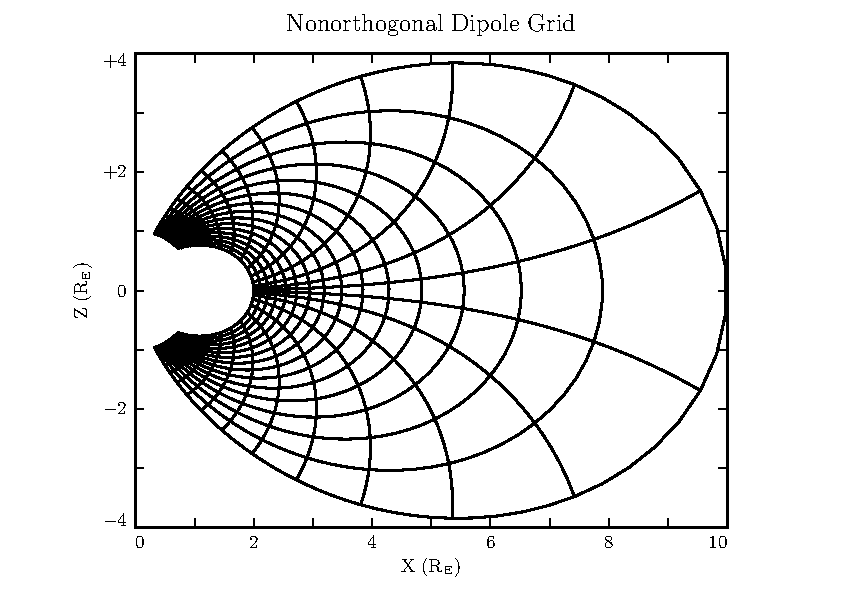
\includegraphics[width=\textwidth]{figures/fig_grid.pdf}
    \caption{
        The model's nonorthogonal grid accommodates both a field-aligned geometry and a constant-height ionospheric boundary. Every fifth point is shown in each direction. The high concentration of grid points near Earth's equator is a consequence of the coordinate system, which converges at the equatorial ionosphere. Earth (not shown) is centered at the origin with unit radius.
    }
    \label{fig_grid}
    \end{center}
\end{figure}

Here, $R$ is the geocentric radius of the ionospheric boundary, taken to be at $R_E + \SI{100}{\km}$, $\theta_0$ is the invariant colatitude, and $r$, $\theta$, and $\phi$ are the usual spherical coordinates.

A thorough discussion of these coordinates, and explicit forms for the resulting basis vectors and metric tensor components can be found in \citet{lysak_2004}. At present, it is sufficient to note that the coordinates are nonorthogonal, and thus have covariant and contravariant basis vectors (${\underline{e}_i \equiv \frac{\partial u^i}{\partial \underline{r}}}$ and ${\underline{e}^i \equiv \frac{\partial \underline{r}}{\partial u^i}}$ respectively) that are not parallel to one another. However, both the covariant and contravariant basis vectors are important to the model.

The basis vectors $\underline{e}^1$, $\underline{e}^2$, and $\underline{e}_3$ are parallel to the usual dipole coordinates, as shown in \cref{to_dipole}, which is the natural basis for the conductivity and dielectric tensors.
\begin{linenomath*}
\begin{align}
    \label{to_dipole}
    \underline{e}^1 &\parallel \hat{x} &
    \underline{e}^2 &\parallel \hat{y} &
    \underline{e}_3 &\parallel \hat{z}
\end{align}
\end{linenomath*}

Where $\hat{z}$ lies along the magnetic field, $\hat{y}$ is azimuthally eastward, and $\hat{x} \equiv \hat{y} \times \hat{z}$ points radially outward at the equator.

In addition, at the ionospheric boundary, $\underline{e}_1$, $\underline{e}_2$, and $\underline{e}^3$ are parallel to the spherical unit vectors:
\begin{linenomath*}
\begin{align}
  \underline{e}_1 &\parallel \hat{\theta} &
  \underline{e}_2 &\parallel \hat{\phi} &
  \underline{e}^3 &\parallel \hat{r}
\end{align}
\end{linenomath*}

As a result, Tuna's grid is aligned everywhere to the zeroth-order dipole magnetic field, while also supporting a fixed-altitude ionospheric boundary.

The results shown in the present work use a grid of 150 values in $u^1$ (150 field lines) and 350 values in $u^3$ (350 grid points per field line). Spacing is on the order of \SI{10}{\km} near the ionosphere and \SI{1000}{\km} at the equator of the outermost field line. The inner boundary is placed at $L = 2$, and the outer boundary at $L = 10$. The time step is determined from the smallest zone crossing time for an Alfve\'n wave, scaled down by a Courant factor of \num{0.1}. Typically, $\delta \! t \sim \SI{10}{\us}$.

% ======================================================================

Like the similar models of \citet{lysak_2013} and \citet{waters_2013}, Tuna can be driven via compression of the simulation's outer boundary -- typically taken as a proxy for solar wind activity. However, the shear and compressional Alfve\'n modes decouple at high $m$, preventing such waves from propagating across magnetic field lines. In order to model noncompressional Pc4 activity at $L\sim5$, it is necessary to inject energy at $L\sim5$.

To this end, Tuna also allows simulations to be driven via modulation of the ring current, a proxy for substorm injection events. For the runs shown, the driving current is spread over a cross section of $\sim\SI{1}{R_E}^2$, centered just outside the plasmapause and just off the equator. In effect, the symmetry in the driver preferentially excites a first-harmonic poloidal wave.

The magnitude of the driving current is estimated from a discrete Fourier transform of the Sym-H storm index during the June 1, 2013 storm. Sym-H is tabulated once per minute, which is too slow to capture activity in the Pc4 band directly. However, a fit of the pink noise spectrum, shown in \cref{fig_symh}, suggests that activity in the Pc4 range could give rise to a field at Earth's surface on the order of \SI{e-2}{\nT}.

This corresponds to a ring current perturbation on the order of \SI{1}{\mega\A}, or $\sim\SI{e-4}{\uA/\m\squared}$ spread over $\sim\SI{1}{\RE}^2$. For the runs shown in the present work, the driving current is azimuthally directed, and its magnitude varies sinusoidally throughout the duration of the run.

\begin{figure}
    \begin{center}
    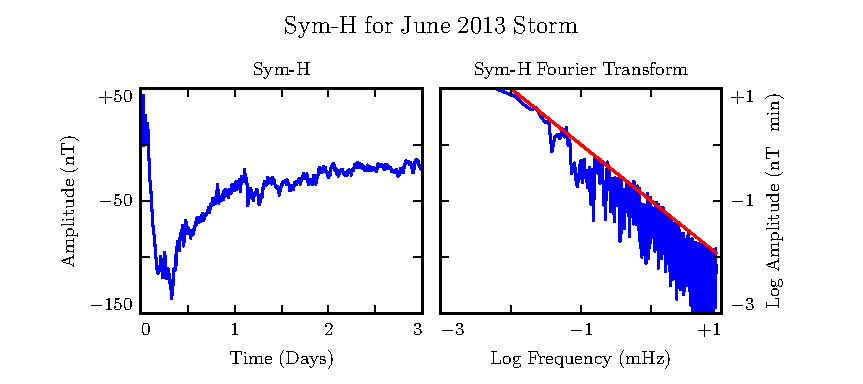
\includegraphics[width=\textwidth]{figures/fig_symh.pdf}
    \caption{
    The left frame shows the Sym-H storm index during the June 2013 storm. On the right is the Fourier transform of that index, scaled to \si{nT}-minutes, along with a fit of the pink noise spectrum, $\frac{ \SI{0.1}{\nT} }{f}$, shown in red. The width of the Pc4 frequency band (\SIrange{7}{25}{\mHz}) is about one inverse minute, suggesting Pc4 contribution to Sym-H of about \SI{e-2}{\nT} at Earth's surface. This suggests \SI{1}{\mega\A} as an appropriate scale for ring current perturbations in the Pc4 range.
    }
    \label{fig_symh}
    \end{center}
\end{figure}

% ======================================================================

Mathematically, the driving current is introduced through an anomalous current term $\underline{J}$ in Amp\`ere's law, apart from the Ohmic current ${\underline{\underline{\sigma}} \cdot \underline{E}}$.

\begin{linenomath*}
\begin{align}
    \label{amp_law}
    \underline{\underline{\epsilon}} \cdot \frac{\partial}{\partial t} \underline{E} &= \frac{1}{\mu_0} \nabla \times \underline{B} - \underline{J}
      - \underline{\underline{\sigma}} \cdot \underline{E}
\end{align}
\end{linenomath*}

Because of the Ohmic current term, the electric field's time derivative in \cref{amp_law} depends on its own future value; $\underline{E}(t + \delta \! t)$ cannot be computed without $\underline{E}(t + \tfrac{\delta \! t}{2})$. This circular dependence is resolved using integrating factors, as discussed in \citet{lysak_2013}. First, the expression is rewritten:
\begin{linenomath*}
\begin{align}
    \label{int_fac}
    \Big( \underline{\underline{\Omega}} + \underline{\underline{ \mathbb{I} }}\frac{\partial}{\partial t} \Big) \cdot
        \underline{E} &= \underline{\underline{V}}^2 \cdot \underline{F}
\end{align}
\end{linenomath*}

Where $\underline{\underline{ \mathbb{I} }}$ is the identity and $\underline{F}$, $\underline{\underline{V}}^2$, and $\underline{\underline{\Omega}}$ are shorthand:
\begin{linenomath*}
\begin{align}
    \underline{F} &\equiv \nabla \times \underline{B} - \mu_0 \underline{J} &
    \underline{\underline{V}}^2 &\equiv \frac{1}{\mu_0} \underline{\underline{\epsilon}}^{-1} &
    \underline{\underline{\Omega}} &\equiv \underline{\underline{\epsilon}}^{-1} \cdot \underline{\underline{\sigma}}
\end{align}
\end{linenomath*}

\cref{int_fac} is then solved by multiplying through by $\exp \left( \underline{\underline{\Omega}} \, t \right)$ (see \citet{hall_2015}), applying the product rule, and integrating over a time step $\delta \! t$.
\begin{linenomath*}
\begin{align}
    \label{amp_final}
    \underline{E} &\leftarrow \exp \left( -\underline{\underline{\Omega}} \, \delta \! t \right) \cdot \underline{E} +
        \delta \! t \, \exp \left( -\underline{\underline{\Omega}} \, \tfrac{\delta \! t}{2} \right) \cdot
        \underline{\underline{V}}^2 \cdot \underline{F}
\end{align}
\end{linenomath*}

Where $\leftarrow$ represents the assignment of a future value based on existing values. If $E$ and $F$ on the right hand side correspond to times $-\frac{\delta \! t}{2}$ and $0$ respectively, the value of $E$ on the left is at time $\frac{\delta \! t}{2}$.

\cref{amp_final} is evaluated by separating the exponential into its diagonal (Pedersen) and off-diagonal (Hall) terms. The Hall terms give a rotation matrix around the magnetic field line, coupling the poloidal and toroidal modes, consistent with \citet{hughes_1974}. Terms proportional to $\exp \left( - \frac{\sigma_0}{\epsilon_0}\delta \! t \right)$ are also present. However, $\frac{\sigma_0}{\epsilon_0}\delta \! t \gtrsim 1000$, so these terms are vanishingly small. As a result, parallel electric fields are taken to be uniformly zero.

Magnetic fields are simply advanced using Faraday's law:
\begin{linenomath*}
\begin{align}
    \label{far_law}
    \frac{\partial}{\partial t} \underline{B} &= - \nabla \times \underline{E}
\end{align}
\end{linenomath*}

For the sake of brevity, the present work does not expand the terms of \cref{amp_final,far_law} in the covariant basis. Those expressions can be found in \citet{mceachern_2016}.

% ======================================================================

Dirichlet and Neumann conditions are applied to the electric and magnetic fields respectively at the inner and outer boundaries; that is, $\underline{E}$ goes to zero at the boundary, as does the spatial derivative of $\underline{B}$. Results of the present work are robust under an exchange of the two.

Between the top of the neutral atmosphere and the bottom of the ionosphere, the model includes a thin, horizontal current sheet at an altitude of \SI{100}{\km} representing the ionosphere's $E$ layer\citep{lysak_2004}. By integrating Amp\`ere's law over the layer, it can be shown\citep{fujita_1988} that the horizontal electric field values at the edge of the grid are determined by the jump in the horizontal magnetic fields:
\begin{linenomath*}
\begin{align}
  \label{jump_condition}
  \underline{\underline{\Sigma}} \cdot \underline{E} &= \frac{1}{\mu_0} \,
    \displaystyle\lim_{\delta \! r \rightarrow 0} \, \bigg[ \, \hat{r} \times \underline{B}
    \, \bigg|^{R_I + \delta \! r}_{R_I - \delta \! r}
\end{align}
\end{linenomath*}

The atmospheric magnetic field is computed in terms of a scalar magnetic potential, $\Psi$, such that $\underline{B}=\nabla \Psi$. The neutral atmosphere is taken to be a perfect insulator, giving $\nabla \times \underline{B}=0$. Combined with $\nabla \cdot \underline{B}=0$ (per Maxwell's equations), this ensures that $\Psi$ satisfies Laplace's equation, $\nabla^2 \Psi = 0$, and thus can be written as a sum of harmonics\citep{jackson_1999}.
\begin{linenomath*}
\begin{align}
  \label{psi_expansion}
  \Psi &= \displaystyle\sum_\ell \left( a_\ell \, r^\ell +
    b_\ell \, r^{-\ell - 1} \right) Y_{\ell m}
\end{align}
\end{linenomath*}

Earth is taken to be a perfect conductor, so $B_r = \frac{\partial}{\partial r} \Psi = 0$ at the surface. In addition, the thin current sheet at the top of the atmosphere is taken to be horizontal, so the radial component of the magnetic field must be the same just above and just below it. Those two boundary conditions (combined with the harmonics' orthonormality) allow solutions for the coefficients $a_\ell$ and $b_\ell$, giving:
\begin{linenomath*}
\begin{align}
  \label{psi_final}
  \begin{split}
  \Psi_E &= \displaystyle\sum_\ell Y_{\ell m} \; \frac{R_I}{ \ell \, \left(\ell - 1\right) } \frac{ \left(2 \ell - 1\right) \, \lambda^\ell }{ 1 - \lambda^{2 \ell + 1} } B_r \cdot Y_{\ell m}^{-1} \\
  \Psi_I &= \displaystyle\sum_\ell Y_{\ell m} \; \frac{R_I}{ \ell \, \left(\ell - 1\right) } \frac{ \left(\ell - 1\right) + \ell \, \lambda^{2 \ell + 1} }{ 1 - \lambda^{2 \ell + 1} } B_r \cdot Y_{\ell m}^{-1}
  \end{split}
\end{align}
\end{linenomath*}

Where $\Psi_E$ and $\Psi_I$ are the values of $\Psi$ at $R_E$ (Earth's surface) and $R_I$ (The bottom of the ionosphere) respectively, $\lambda \equiv \frac{R_E}{R_I} \sim \num{0.975}$, and $B_r \cdot Y_{\ell m}^{-1} \equiv \displaystyle\sum_i B_r [i] \; Y_{\ell m}^{-1} \! [i]$.

Magnetic field values at the top of the atmosphere are used to compute electric field boundary conditions via \cref{jump_condition}. Those at Earth's surface are output, suitable for comparison with magnetometer data.

% ######################################################################

\section{Numerical Results}

The present section discusses the numerical resuts shown in \cref{fig_brms,fig_energy,fig_layers_day,fig_layers_night,fig_ground_day,fig_ground_night}. In each figure, an lattice of plots shows a side-by-side comparison of an ensemble of runs conducted with Tuna.

In \cref{fig_brms}, the distributions of magnetic field perturbations are shown for four \SI{300}{\second} runs conducted with Tuna using a dayside ionospheric profile and \SI{22}{\mHz} driving throughout the duration of the run. Each column shows a different value of $m$ (1, 4, 16, and 64), while the rows show RMS poloidal, toroidal, and compressional magnetic field strengths. At low $m$ (left), the three components are comparable in magnitude; as $m$ increases (to the right), the compressional component becomes appreciably weaker and the distribution of energy appears more guided. Toroidal wave activity is concentrated near resonant $L$ shells, while poloidal activity is spread more broadly -- particularly at low $m$.

\begin{figure}
    \begin{center}
    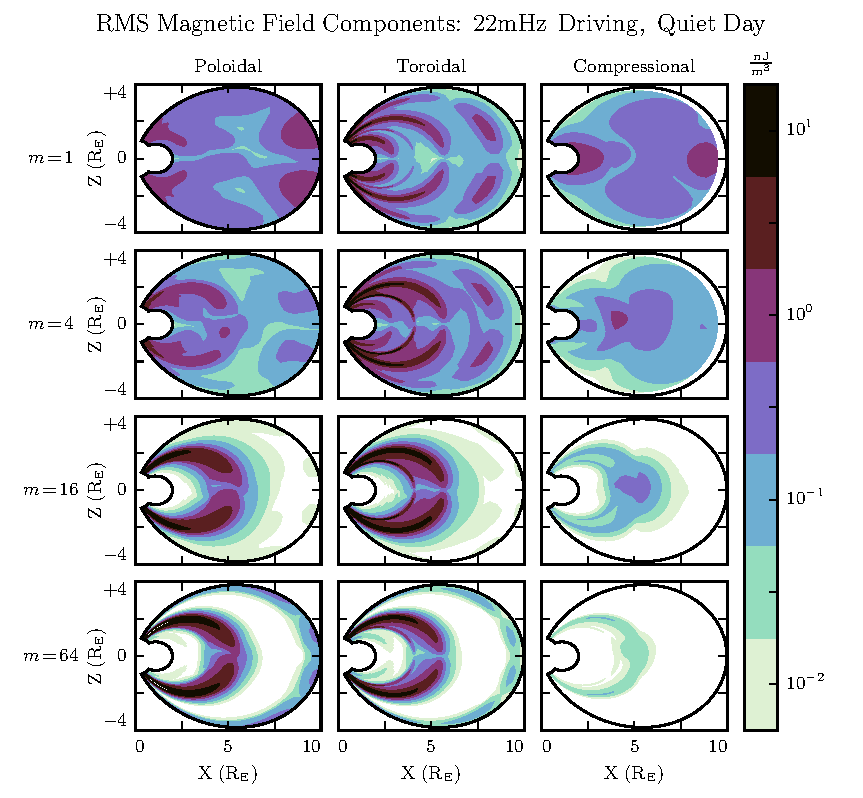
\includegraphics[width=\textwidth]{figures/fig_brms.pdf}
    \caption{
        Each cell in the above figure shows root-mean-square magnetic field perturbations over the course of a \SI{300}{\s} run. The four columns show four different runs, with azimuthal modenumbers 1, 4, 16, and 64 respectively. The rows show poloidal, toroidal, and compressional magnetic field components. At low $m$, compressional activity is apparent by the fact that all three components are comparable in magnitude; as $m$ increases, compressional activity diminishes. Poloidal waves are spread broadly in $L$ at low $m$, becoming guided only as large $m$ prevents energy from moving across field lines. In contrast, toroidal waves are sharply defined in $L$ regardless of $m$.
    }
    \label{fig_brms}
    \end{center}
\end{figure}

Those same four runs are shown in the top row of \cref{fig_energy}, resolved in time rather than in space. The total energy in the toroidal wave is shown in red, and the total energy in the poloidal wave is shown in blue; see \cref{energy_eqn}. The second row is analogous, but uses the nightside ionospheric profile and drives at \SI{16}{\mHz} (the ionospheric profile significantly affects the ionosphere's Alfve\'n speed, and thus resonant frequencies). Each subplot is analogous to Figure 3 in \citet{mann_1995}.
\begin{linenomath*}
\begin{align}
  \label{energy_eqn}
    U_P &= \frac{1}{2} \displaystyle\int dV \; \frac{1}{\mu_0} B_x^2 + \epsilon_\bot E_y^2 \\
    U_T &= \frac{1}{2} \displaystyle\int dV \; \frac{1}{\mu_0} B_y^2 + \epsilon_\bot E_x^2
\end{align}
\end{linenomath*}

Since all driving is injected into the poloidal mode, the presence of any toroidal wave shows that energy converts between modes; the conversion is clearly slower for runs with larger $m$ values; and the conversion seems to be asymptotic, rather than oscillatory. These properties are all consistent with \citet{mann_1995}.

Whereas past work made use of an initial wave and a perfectly-conducting boundary, the present work leverages ongoing driving and a realistic, height-resolved conductivity profile. In particular, \cref{fig_energy} allows a comparison of energy accumulation on the dayside and on the nightside in response to the same energy input. On the dayside, where conductivity is high, the toroidal mode grows in magnitude over the course of many drive periods. Conversely, on the nightside, the driving and dissipation timescales are comparable, so the system quickly comes to a steady state. This suggests that poloidal waves are effective drivers of (same-harmonic) toroidal waves on the dayside, and are less effective as drivers of nightside toroidal activity.

\begin{figure}
    \begin{center}
    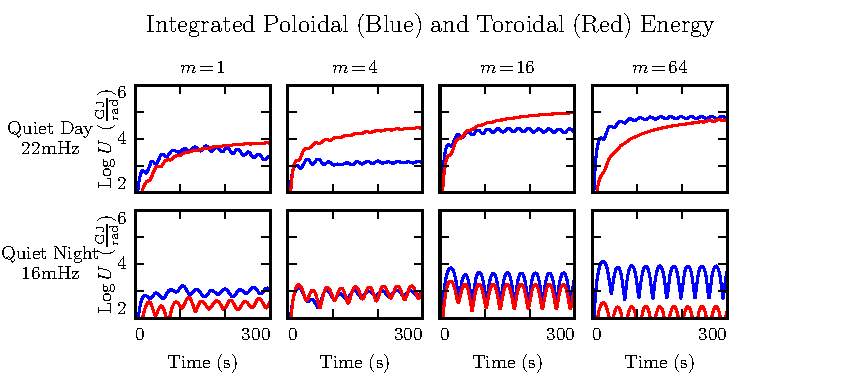
\includegraphics[width=\textwidth]{figures/fig_energy.pdf}
    \caption{
        Each cell above shows integrated poloidal (blue) and toroidal (red) energy as a function of time for a single run. The top row shows runs using a dayside ionospheric profile (driven at \SI{22}{\mHz}), and the bottom row nightside (driven at \SI{16}{\mHz}). Driving is purely poloidal, and energy converts over time to the toroidal mode. On the dayside, it is clear that energy converts faster when $m$ is smaller, consistent with the findings of \citet{mann_1995}. On the nightside, the dissipation timescale is comparable to the conversion timescale; despite the fact that energy is continuously injected into the system via the driving current, there is no long-term accumulation of energy in the toroidal or poloidal mode.
    }
    \label{fig_energy}
    \end{center}
\end{figure}

Another view of the dayside (\cref{fig_energy} top row) and nightside (\cref{fig_energy} bottom row) runs is shown in \cref{fig_layers_day,fig_layers_night} respectively.

Time and $L$ are shown on the horizontal and vertical axes; contours indicate mean energy density over that $L$-shell.

On the dayside (\cref{fig_layers_day}), at low $m$, energy is able to move freely across magnetic field lines, even escaping the simulation domain. Poloidal energy is not localized for long enough to build up a strong resonance in any particular place, or for much energy to convert to the toroidal mode. (Note that the buildup of poloidal energy at $m = 1$, $L > 8$ is likely nonphysical, due to a third harmonic very close to the simulation boundary.) As $m$ increases, energy is less able to cross field lines; both toroidal and poloidal resonances are strongest when $m$ is highest.

\begin{figure}
    \begin{center}
    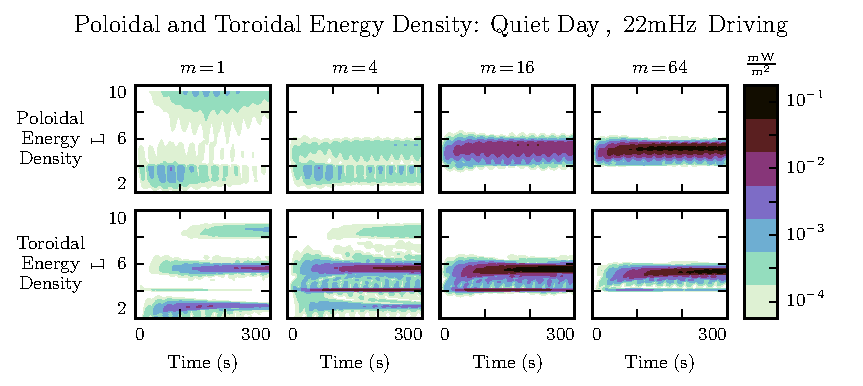
\includegraphics[width=\textwidth]{figures/fig_layers_day.pdf}
    \caption{
        Above are the same runs shown in the top row of \cref{fig_energy}; the runs are the same except that $m$ increases to the right. Rather than show the energy integrated over the whole simulation domain, the above figure shows energy density, with time on the horizontal axis and $L$ on the vertical axis. The top and bottom rows show poloidal and toroidal energy distributions respectively. Toroidal activity is shown to be sharply concentrated at resonant $L$ shells; it is strongest at high $m$ because that's where energy converts most effectively from the poloidal mode. Poloidal waves are spread broadly in $L$. At low $m$, some energy escapes the simulation domain entirely. Poloidal waves appear sharp only when high $m$ prevents energy from spreading.
    }
    \label{fig_layers_day}
    \end{center}
\end{figure}


The behavior on the nightside (\cref{fig_layers_night}) is in several ways similar to that on the dayside, but the result looks much different due to the lower ionospheric conductivity. At low $m$, energy moves freely in $L$, even escaping the simulation. At high $m$ waves are guided, allowing energy to convert from the poloidal mode into a localized toroidal mode. However, due to the fast dissipation timescale, the strongest toroidal mode on the nightside is not at $m = 64$, where guiding is strongest, but at $m = 16$, where the strength of the guiding strikes a balance with the rate of poloidal-to-toroidal conversion.

\begin{figure}
    \begin{center}
    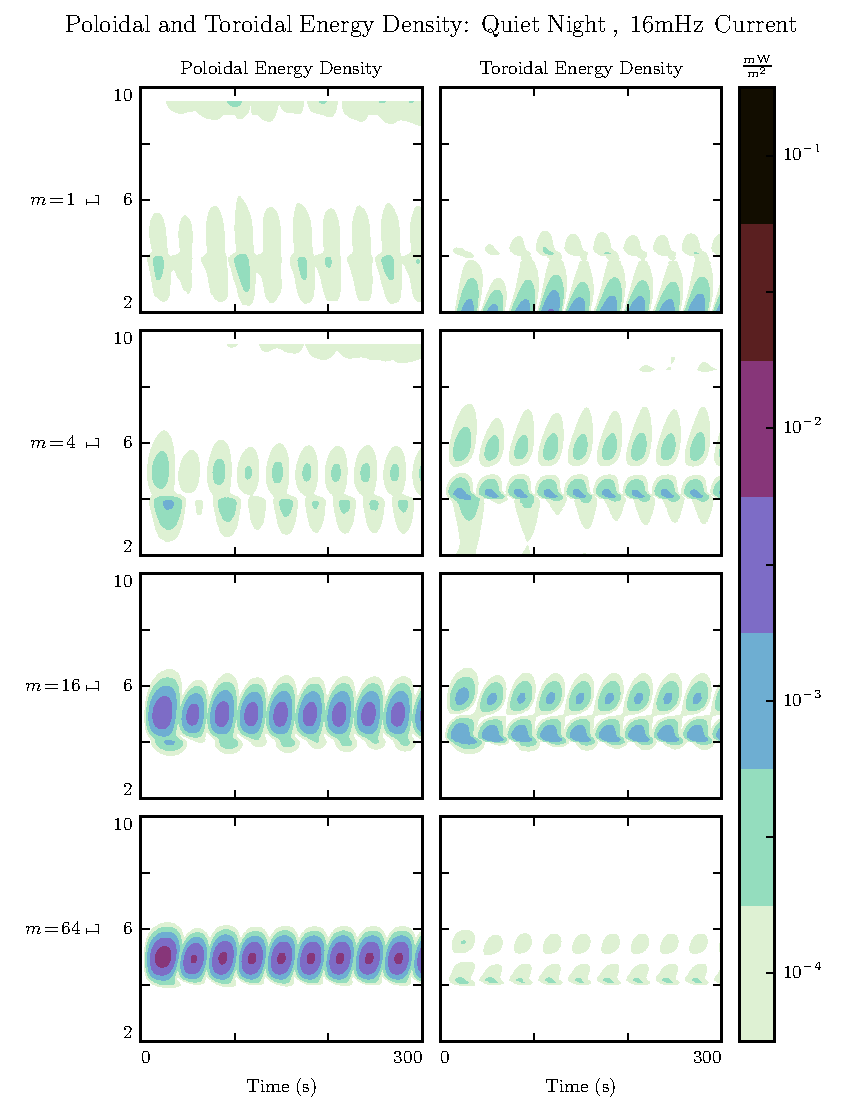
\includegraphics[width=\textwidth]{figures/fig_layers_night.pdf}
    \caption{
        The above figure is analogous to \cref{fig_layers_day}, except that it shows runs carried out using a nightside ionospheric profile instead of dayside. Four runs are shown, each at a different $m$, and the rows show poloidal and toroidal energy density as a function of $L$ and time. In a general sense, the behavior matches that seen on the dayside: poloidal activity is broad in $L$ while toroidal waves appear only where resonant. The difference is in the wave magnitude. The ongoing driving current is the same between the dayside and nightside runs, but the response on the nightside is smaller by an order of magnitude due to increased Joule dissipation.
    }
    \label{fig_layers_night}
    \end{center}
\end{figure}

A final angle on those same eight simulations is shown in \cref{fig_ground_day,fig_ground_night}: their magnetic signatures at Earth's surface. Due to the effect of the ionosphere, note that $B_\phi$ corresponds to the poloidal mode, and $B_\theta$ to the toroidal mode. Maximum amplitude is indicated wherever it exceeds \SI{3}{\nT}.

\begin{figure}
    \begin{center}
    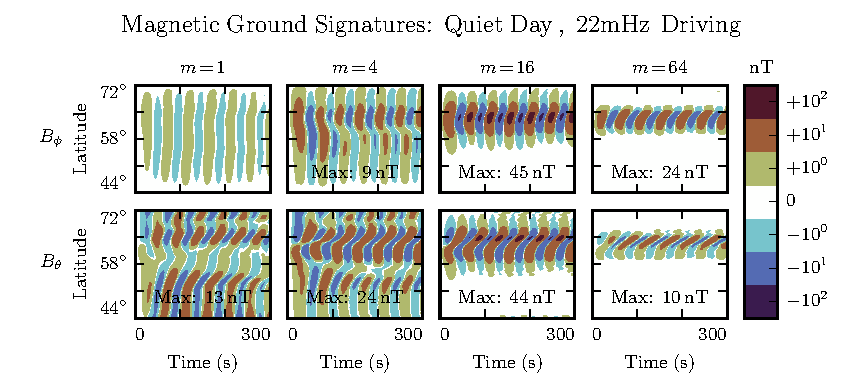
\includegraphics[width=\textwidth]{figures/fig_ground_day.pdf}
    \caption{
        The magnetic ground signatures are shown for the same runs as in previous figures. Ground signatures at low $m$ are weak because the waves in space are weak. Ground signatures at high $m$ are attenuated before reaching ground magnetometers. The two effects combine to create a maximum at $m \sim 16$. The maximum ground signatures consistently appear in the east-west magnetic field component, corresponding to the poloidal mode. Careful examination shows furthermore that the events are clockwise to an observer above $\sim\SI{65}{\degree}$ and counterclockwise to an observer below. All of these properties are commonly ascribed to giant pulsations.
    }
    \label{fig_ground_day}
    \end{center}
\end{figure}

At low $m$, ground signatures are weak and diffuse in latitude because the waves in space are weak and diffuse. At high $m$, ground signatures are more sharply defined, but are also attenuated by the atmosphere. The strongest ground signatures are visible at $m = 16$ (note that further investigation, not shown, finds that ground signatures at $m = 32$ are comparable in strength to those at $m = 16$, and those at $m = 8$ are not). The strongest peaks are in $B_\phi$, corresponding to the poloidal mode. Furthermore, the events display a chirality flip between their top and bottom halves; this is particularly apparent on the nightside. The phase of $B_\theta$ leads that of $B_\phi$ at high latitude, and lags it at low latitude.

\begin{figure}
    \begin{center}
    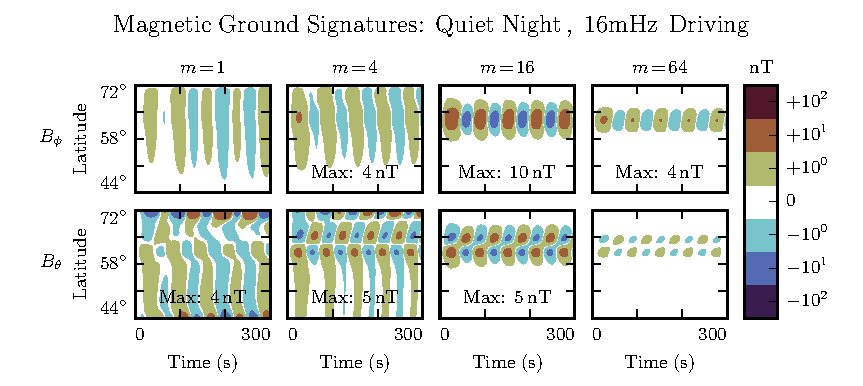
\includegraphics[width=\textwidth]{figures/fig_ground_night.pdf}
    \caption{
        Above are the ground signatures for the four nightside runs. As on the dayside, shown in \cref{fig_ground_day}, magnetic fields at Earth's surface are strongest when $m \sim 16$, and peak signals correspond to the poloidal mode. Compared to the dayside, ground signatures on the nightside are weaker, and the chirality shift (clockwise to the north and counterclockwise to the south) is much clearer.
    }
    \label{fig_ground_night}
    \end{center}
\end{figure}

The findings together suggest that the morphology of giant pulsations reveals relatively little about their origins. One can consider a hypothetical magnetosphere subject to constant driving: broadband in frequency, broadband in modenumber, just outside the plasmapause. Low-$m$ poloidal waves will quickly propagate away, contributing little energy to the toroidal mode. High-$m$ waves will resonate in place, accumulating energy over time, and give rise to ``multiharmonic toroidal waves'' (per \citet{takahashi_2011}); Fourier components that do not match the local eigenfrequency will accumulate energy over just a few wave periods before reaching asymptotic values. Waves with very high modenumbers will be attenuated by the ionosphere. The response on the ground will be counterclockwise at low latitude, clockwise at high latitude, peaked at modenumbers of 16 to 32, and mostly east-west polarized. In other words, the measurements will look very much like a giant pulsation.

The present results offer no explanation as to the tendency of giant pulsations to drift azimuthally, or to appear pre-dawn in MLT --- though the latter is addressed by the observational results in below.

% ######################################################################

\section{Van Allen Probes Observations}

The present section gives a survey of 762 thirty-minute Pc4 events, each characterized in terms of both parity and polarization, and selected in a way that does not introduce an apparent bias in either property. No past study has so thoroughly disentangled the parity and polarization of these waves.

Events are selected from Van Allen Probe data collected between October 2012 and August 2015. Between the two probes, that's just over 2000 days of observation. The two probes are taken to be independent observers. A preliminary estimate shows that Pc4 events are sufficiently short-lived and narrow in MLT that the same event is rarely ($\sim\SI{1}{\percent}$) observed by both probes.

%\todo{Per Aaron: ``Level 3" doesn't have any meaning to most scientists. Be more specific about what quantities you're using}

Electric and magnetic field data are collected using the probes' EFW\citep{wygant_2013} and EMFISIS\citep{kletzing_2013} instruments respectively. Level 3 (inertial) values are used, averaged over the $\sim\SI{11}{\second}$ probe spin period. Three-dimensional electric field data is obtained by using the $\underline{E} \cdot \underline{B} = 0$ assumption. This method is reliable only when there is a significant offset between the magnetic field and the probe's spin plane. Data for which the spin plane and the magnetic field fall within \SI{15}{\degree} of each other -- about half -- is discarded, potentially introducing a sampling bias with respect to MLT and/or geomagnetic conditions. The spatial distribution of three-dimensional electric and magnetic fields data is shown in \cref{fig_pos}. The data set includes about one and a half precessions around Earth, meaning there is twice as much sampling (at apogee) of the nightside as there is on the dayside.

\begin{figure}
    \begin{center}
    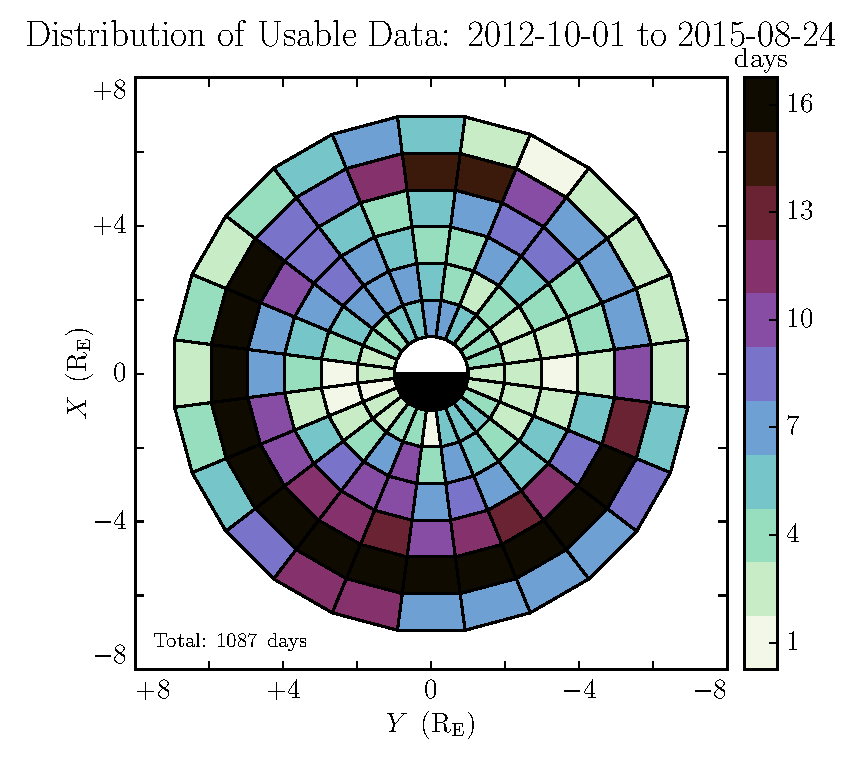
\includegraphics[width=\textwidth]{figures/fig_pos.pdf}
    \caption{
        The above figure shows the distribution of data collected by the Van Allen Probes for which 3D electric and magnetic fields are available. (When the probe's axis aligns too closely with the magnetic field, the 3D electric field cannot be determined reliably.) Coverage is lopsided because the probes had completed one and a half precessions around Earth; that is, the nightside is double-sampled at apogee. Coverage is good outside $L\sim4$; note that each day of sampling is broken down into 48 half-hour events.
    }
    \label{fig_pos}
    \end{center}
\end{figure}

Field measurements are transformed into the same dipole coordinates used above to describe the numerical model. The $z$ axis is set to align with the background magnetic field, which is estimated using a ten-minute running average of the magnetic field measurements. The $y$ axis is set parallel to $\hat{z} \times \underline{r}$, where $\underline{r}$ is the probe's geocentric position vector. The $x$ axis is then defined per $\hat{x} \equiv \hat{y} \times \hat{z}$. This scheme guarantees that the axes are right-handed and pairwise orthogonal\citep{liu_2009}.

The $\sim1000$ days of usable data are considered half an hour at a time, which gives a frequency resolution of $\sim\SI{0.5}{\mHz}$ in the discrete Fourier transform. Spectra are computed for all six field components: $\overset{\sim}{B_x}$, $\overset{\sim}{B_y}$, $\overset{\sim}{B_z}$, $\overset{\sim}{E_x}$, $\overset{\sim}{E_y}$, and $\overset{\sim}{E_z}$. The background
magnetic field is subtracted before transforming the magnetic field components, leaving only the perturbation along each axis. A DC offset is also applied to each waveform so that its mean over the event is zero.

Poynting flux along the field is computed from the electric and magnetic field transforms, then scaled by a factor of $\left( \frac{r}{R_I} \right)^3$. This factor compensates for flux tube compression by assuming the Poynting flux integrated over the flux tube is independent of altitude. As a result, all Poynting flux values are effective at the ionosphere, mitigating bias due to measurement potition. Poloidal and toroidal Poynting flux are given by:
\begin{linenomath*}
\begin{align}
    \overset{\sim}{S_P} &\equiv -\left( \frac{r}{R_I} \right)^3\frac{1}{\mu_0} \overset{\sim}{E_y} \overset{\sim}{B_x^*} &
    \overset{\sim}{S_T} &\equiv  \left( \frac{r}{R_I} \right)^3\frac{1}{\mu_0} \overset{\sim}{E_x} \overset{\sim}{B_y^*}
\end{align}
\end{linenomath*}

An example event, showing electric and magnetic field measurements as well as real and imaginary Poynting flux spectra, is shown in \cref{fig_event}.

\begin{figure}
    \begin{center}
    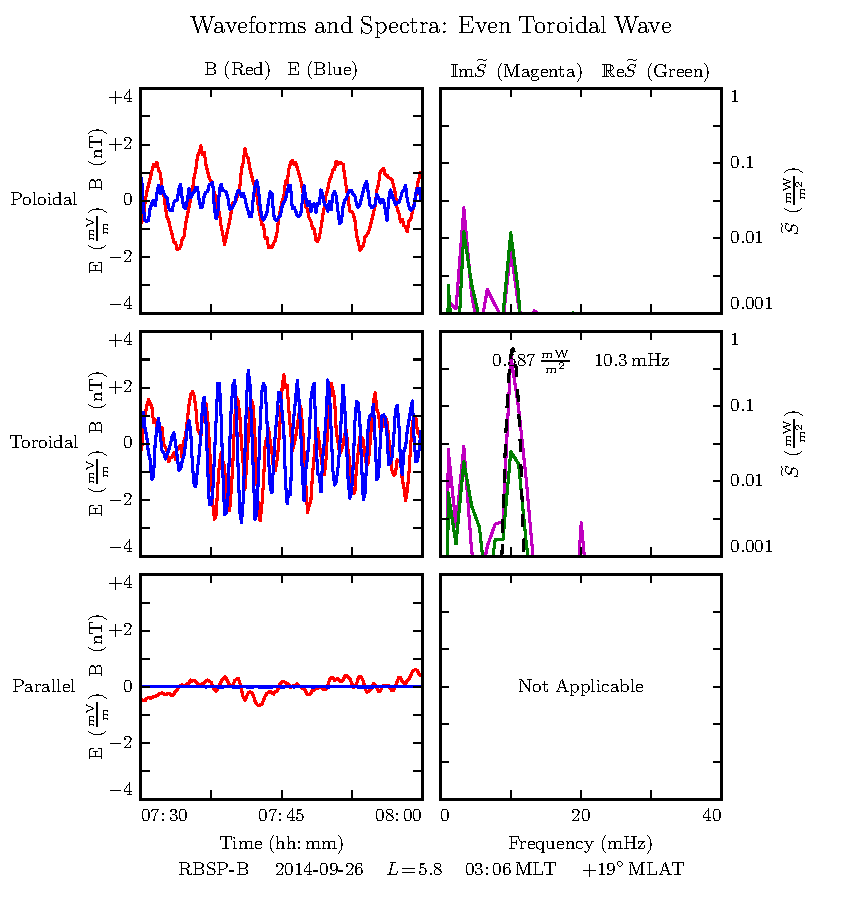
\includegraphics[width=\textwidth]{figures/fig_event.pdf}
    \caption{
        An example half-hour event is shown. On the left are electric and magnetic field measurements. On the right are the real and imaginary components of the corresponding Poynting flux spectra. The black dotted line shows a Gaussian fit of the Poynting flux magnitude. A toroidal wave is evident at \SI{10.3}{\mHz}. The poloidal channel also shows activity near \SI{10}{\mHz}; however, no poloidal event is selected due to the comparably-strong oscillation at \SI{3}{\mHz}. The \SI{3}{\mHz} oscillation is an artifact of a thruster firing roughly 12 hours earlier.
    }
    \label{fig_event}
    \end{center}
\end{figure}

The poloidal and toroidal channels are independently checked for Pc4 waves. For each channel, a Gaussian profile is fit to the magnitude of the Poynting flux, $|\overset{\sim}{S}\left(\omega\right)|$. If the fit fails to converge, or if the peak of the Gaussian does not fall within \SI{5}{\mHz} of the peak value of $\overset{\sim}{S}$, the event is discarded. Events are also discarded if their frequencies fall outside the Pc4 frequency range (\SIrange{7}{25}{\mHz}) or if their amplitudes fall below \SI{0.01}{\mW/\m\squared} (out of consideration for instrument sensitivity). The magnitude threshold is set in Poynting flux instead of magnetic field (which is more typical) in an effort to reduce bias in event selection. When events are selected based on the magnitude of the wave magnetic field, first-harmonic waves become more difficult to detect, due to their magnetic field node at the equator\citep{dai_2015}.

In order to distinguish an odd mode from an even mode\footnote{
The techniques used in the present work do not make an explicit distinction between first (second) harmonics and higher odd (even) harmonics. That said, higher harmonics are comparably rare in the inner magnetosphere, so it is reasonable to assume that odd events are mostly first harmonics and even events are mostly second harmonics.}, it is necessary to know whether the observation is made north or south of the equator. Any event within \SI{3}{\degree} of the magnetic equator is discarded to avoid misclassification. Parity classification also requires an identifiable phase shift between the electric and magnetic fields; if an event's electric and magnetic fields are not coherent at a level of 0.9 or better (judged at the discrete Fourier transform point closest to the peak of the Gaussian fit) then the event is also discarded.

A visual inspection of events shows that those with broad ``peaks'' in their spectra are typically bad fits of noisy or multiharmonic data. A threshold is set at a FWHM of \SI{3}{\mHz} (equally, a standard deviation of \SI{1.27}{\mHz}). Any event with a Gaussian fit broader than that is discarded.

Roughly speaking, event distributions (shown in \cref{fig_all,fig_mode}) are found to be consistent with past surveys. Toroidal events dominate overall, and are primarily seen on the morning side. Poloidal events are spread broadly in MLT with a peak near noon and distinctive odd harmonics in the early morning. From there, the simultaneous consideration of harmonic and polarization, combined with the numerical results above, offers significant insight.

\begin{figure}
    \begin{center}
    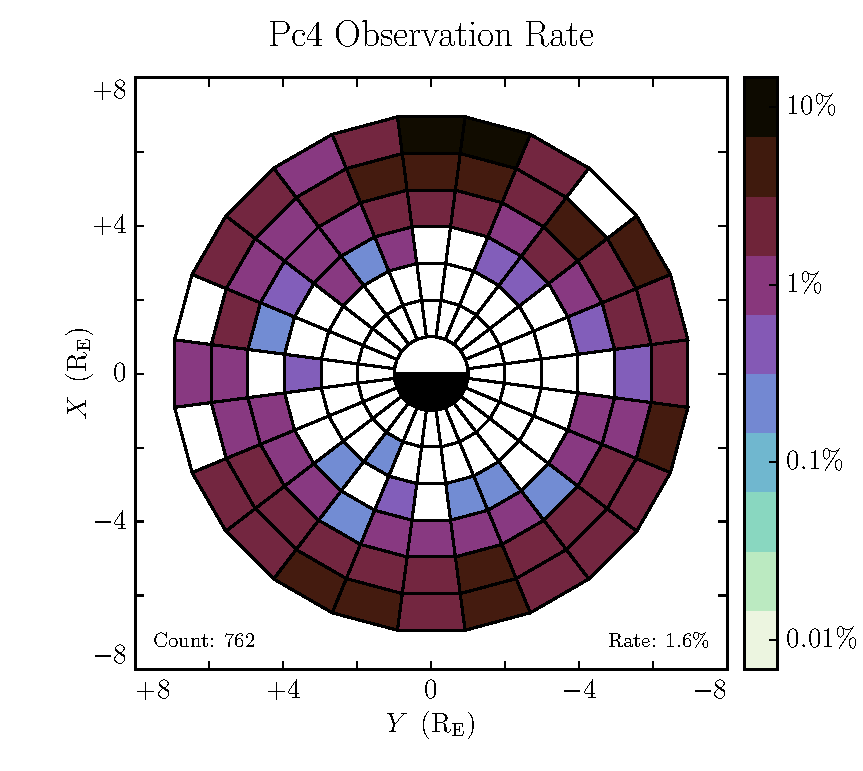
\includegraphics[width=\textwidth]{figures/fig_all.pdf}
    \caption{
        The above figure shows the spatial distribution of all 762 observed Pc4 events. Counts are normalized by the amount of usable data in each bin. The value in the bottom-right corner is the average of all bin rates, weighted by bin area. Bins shown in white contain zero events.
    }
    \label{fig_all}
    \end{center}
\end{figure}

The near-noon peak of poloidal Pc4 events is shown to be due to even events (a majority subset). Odd poloidal events occur preferentially near midnight and across the morning side. Toroidal events are mostly odd, and it is specifically the odd toroidal events which occur on the morningside, while even toroidal events peak near noon.

The spatial distribution of even poloidal events looks much like the spatial distribution of even toroidal events; both distributions peak near noon, and both prefer the evening side to the morning side. The primary difference between them is that the toroidal events are more sharply peaked near noon, while the poloidal events spread more broadly across the afternoon and evening. Similarly, odd poloidal and odd toroidal events exhibit similar distributions with the toroidal distribution skewed slightly dayward. This is consistent (per the above numerical results) with poloidal events as an effective source for (same-parity) toroidal events on the dayside, and a less-effective source on the nightside.

\begin{figure}
    \begin{center}
    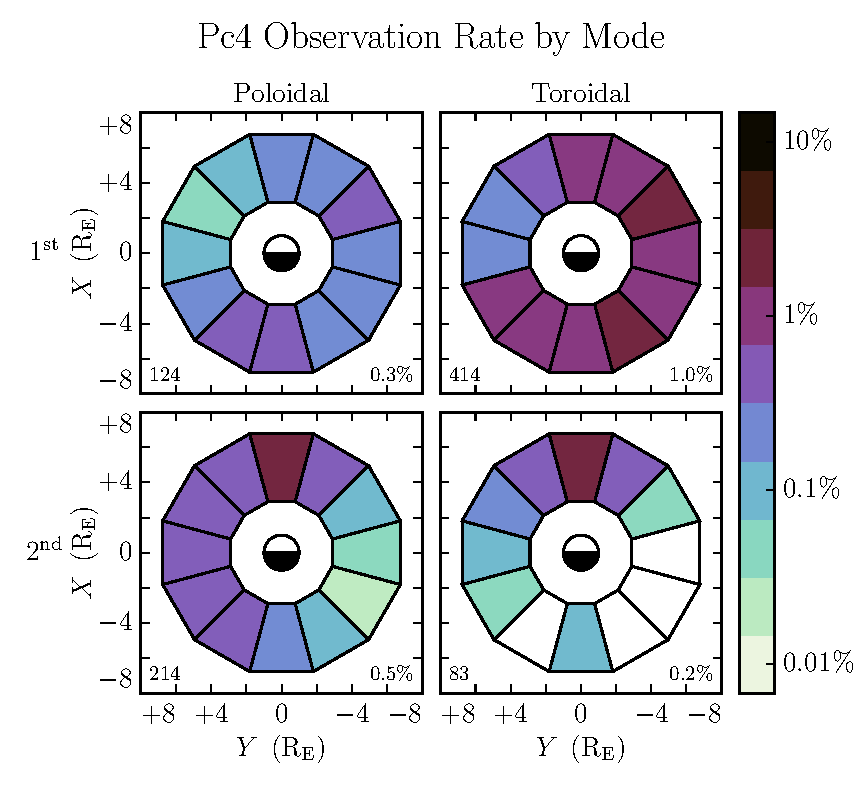
\includegraphics[width=\textwidth]{figures/fig_mode.pdf}
    \caption{
        The above figure shows the spatial distribution for the same 762 events shown in \cref{fig_all}, partitioned by polarization and parity. The selection criteria ensure that both properties are known for each event. Event counts are normalized by the time spent by the amount of usable data in each bin. Events for which a wave is present in both the poloidal and toroidal channels is shown in both distributions; there are 54 such events.
    }
    \label{fig_mode}
    \end{center}
\end{figure}

As a corrolary, the distribution of odd poloidal events is found to closely resemble the distribution of giant pulsations: midnight and morning. This (consistent with the numerical results) suggests that the distinctive properties attributed to giant pulsations are in fact shared by odd poloidal Pc4s overall.

Curiously, odd toroidal events are found to occur at a higher rate than even ones, while the opposite is true for poloidal events. This disparity may offer clues to the source of these waves, or hint at a harmonic dependence in the rate of poloidal-to-toroidal conversion.

%\todo{Do we want to get into event phase? Scott says: Ask Bob. Aaron says: If you want to get into phase, move details to an appendix.}

% ######################################################################

\section{Discussion}

The present work discusses the development of Tuna, a numerical model created with Pc4s in mind. Using Tuna, Pc4s are modeled across varying frequencies, azimuthal modenumbers, and ionospheric conductivity profiles, suggesting novel connections between several properties. Numerical results are complemented by a survey of Pc4 events measured by the Van Allen Probes.

Numerical work suggests that poloidal Pc4s convert to the toroidal mode on timescales comparable to the oscillation period, suggesting poloidal waves as a significant source for toroidal waves. On the nightside, the dissipation timescale is comparable to the oscillation period as well, so much poloidal energy is lost before converting to the toroidal mode.

Numerical results also suggest that the distinctive ground signatures attributed to giant pulsations may be features of first-harmonic poloidal Pc4s overall. Generic first harmonic poloidal waves are shown to exhibit peak ground signatures around ${m = 16}$, which are sharply peaked at auroral latitudes, and which occur preferrentially during times of quiet solar activity.

The present results are limited to a first-harmonic, sinusoidal, poloidal driver; however, Tuna has the capacity to deliver more interesting driving waveforms as well, and higher harmonics could be added with trivial modifications to the code.

% -----------------------------------------------------------------------------

Using data from the Van Allen Probes EMFISIS and EMF instruments, a survey of 762 half-hour Pc4 events is presented with each event classified by both polarization and harmonic.

Odd poloidal events are shown to be concentrated from midnight through the morning --- as with the numerical results, it seems that giant pulsations are unusual when compared to Pc4s overall, but not compared to odd poloidal Pc4s specifically.

Odd toroidal events exhibit a similar distribution to odd poloidal events, but are skewed dayward across the morningside. The same is true for even events: even poloidal events peak at noon and are spread across the evening side, while even toroidal events peak at noon and are far less spread. These distributions are consistent with the poloidal mode as a significant source for same-harmonic toroidal events, particularly on the dayside, as suggested by the numerical results.

Overall, poloidal and toroidal events exhibit disparate distributions because poloidal events are primarily even, while toroidal events are mostly odd; the cause is not apparent.

The body of Pc4 events available in Van Allen Probe data is growing over time. After the probes complete their second precession, event statistics on the dayside should improve considerably. Furthermore, the present work considers the two Van Allen Probes to be independent observers, but future work could look into the few Pc4 events which are observed simultaneously (or in quick succession) by both probes.

% ######################################################################

\appendix

\section{Appendix}

The source code for Tuna is available at \texttt{https://github.com/UMN-Space-Physics}, as are the scripts used to process the Van Allen Probes data.

% ######################################################################

\acknowledgments

This work was aided by discussions with Cynthia Cattell, Tom Jones, Lindsay Glesener, Yan Song, and Sheng Tian. Funding came from the Office of the Vice President for Research at the University of Minnesota, as well as NSF grant AGS-1405383 and NASA grant NNX12AD14G. Supercomputer resources were provided by the Minnesota Supercomputing Institute. Travel support was provided in part by GEM.

Van Allen Probes data is available via the Van Allen Probes Science Gateway.

% ######################################################################

\begin{thebibliography}{50}
\providecommand{\natexlab}[1]{#1}
\expandafter\ifx\csname urlstyle\endcsname\relax
  \providecommand{\doi}[1]{doi:\discretionary{}{}{}#1}\else
  \providecommand{\doi}{doi:\discretionary{}{}{}\begingroup
  \urlstyle{rm}\Url}\fi

\bibitem[{\textit{Anderson et~al.}(1990)\textit{Anderson, Engebretson, Rounds,
  Zanetti, and Potemra}}]{anderson_1990}
Anderson, B.~J., M.~J. Engebretson, S.~P. Rounds, L.~J. Zanetti, and T.~A.
  Potemra (1990), A statistical study of {Pc} 3-5 pulsations observed by the
  {AMPTE}/{CCE} magnetic fields experiment, 1. occurrence distributions,
  \textit{J. Geophys. Res.}, \textit{95}(A7), 10,495,
  \doi{10.1029/ja095ia07p10495}.

\bibitem[{\textit{Angelopoulos}(2008)}]{angelopoulos_2008}
Angelopoulos, V. (2008), The {THEMIS} mission, \textit{Space Science Reviews},
  \textit{141}(1-4), 5--34, \doi{10.1007/s11214-008-9336-1}.

\bibitem[{\textit{Birkeland}(1901)}]{birkeland_1901}
Birkeland, K. (1901), Exp{\'e}dition norv{\'e}gienne de 1899-1900 pour
  l'{\'e}tude des aurores bor{\'e}ales, \textit{Mat. Naturvidensk. Kl.},
  \textit{KI}(I).

\bibitem[{\textit{Brekke et~al.}(1987)\textit{Brekke, Feder, and
  Berger}}]{brekke_1987}
Brekke, A., T.~Feder, and S.~Berger (1987), Pc4 giant pulsations recorded in
  {Troms{\o}}, 1929-1985, \textit{Journal of Atmospheric and Terrestrial
  Physics}, \textit{49}(10), 1027--1032, \doi{10.1016/0021-9169(87)90109-7}.

\bibitem[{\textit{Chen and Hasegawa}(1974)}]{chen_1974}
Chen, L., and A.~Hasegawa (1974), A theory of long-period magnetic pulsations:
  1. steady state excitation of field line resonance, \textit{J. Geophys.
  Res.}, \textit{79}(7), 1024--1032, \doi{10.1029/ja079i007p01024}.

\bibitem[{\textit{Chisham and Orr}(1991)}]{chisham_1991}
Chisham, G., and D.~Orr (1991), Statistical studies of giant pulsations (pgs):
  Harmonic mode, \textit{Planetary and Space Science}, \textit{39}(7),
  999--1006, \doi{10.1016/0032-0633(91)90105-j}.

\bibitem[{\textit{Cummings et~al.}(1969)\textit{Cummings, O'Sullivan, and
  Coleman}}]{cummings_1969}
Cummings, W.~D., R.~J. O'Sullivan, and P.~J. Coleman (1969), Standing
  {Alfv{\'e}n} waves in the magnetosphere, \textit{J. Geophys. Res.},
  \textit{74}(3), 778--793, \doi{10.1029/JA074i003p00778}.

\bibitem[{\textit{Dai et~al.}(2013)\textit{Dai, Takahashi, Wygant, Chen,
  Bonnell, Cattell, Thaller, Kletzing, Smith, MacDowall, Baker, Blake, Fennell,
  Claudepierre, Funsten, Reeves, and Spence}}]{dai_2013}
Dai, L., K.~Takahashi, J.~R. Wygant, L.~Chen, J.~Bonnell, C.~A. Cattell,
  S.~Thaller, C.~Kletzing, C.~W. Smith, R.~J. MacDowall, D.~N. Baker, J.~B.
  Blake, J.~Fennell, S.~Claudepierre, H.~O. Funsten, G.~D. Reeves, and H.~E.
  Spence (2013), Excitation of poloidal standing {Alfv{\'e}n} waves through
  drift resonance wave-particle interaction, \textit{Geophys. Res. Lett.},
  \textit{40}, 4127--4132, \doi{10.1002/grl.50800}.

\bibitem[{\textit{Dai et~al.}(2015)\textit{Dai, Takahashi, Lysak, Wang, Wygant,
  Kletzing, Bonnell, Cattell, Smith, MacDowall, Thaller, Breneman, Tang, Tao,
  and Chen}}]{dai_2015}
Dai, L., K.~Takahashi, R.~Lysak, C.~Wang, J.~R. Wygant, C.~Kletzing,
  J.~Bonnell, C.~A. Cattell, C.~W. Smith, R.~J. MacDowall, S.~Thaller,
  A.~Breneman, X.~Tang, X.~Tao, and L.~Chen (2015), Storm time occurrence and
  spatial distribution of {Pc4} poloidal {ULF} waves in the inner
  magnetosphere: A {Van Allen Probes} statistical study, \textit{J. Geophys.
  Res. Space Physics}, \textit{120}, 4748--4762, \doi{10.1002/2015JA021134}.

\bibitem[{\textit{Degeling et~al.}(2014)\textit{Degeling, Rankin, and
  Zong}}]{degeling_2014}
Degeling, A.~W., R.~Rankin, and Q.-G. Zong (2014), Modeling radiation belt
  electron acceleration by {ULF} fast mode waves, launched by solar wind
  dynamic pressure fluctuations, \textit{J. Geophys. Res. Space Physics},
  \textit{119}(11), 8916--8928, \doi{10.1002/2013ja019672}.

\bibitem[{\textit{Eleman}(1967)}]{eleman_1967}
Eleman, F. (1967), Studies of giant pulsations, continuous pulsations, and
  pulsation trains in the geomagnetic field, \textit{Ark. Geofys.}, \textit{5},
  231--282.

\bibitem[{\textit{Elkington}(2003)}]{elkington_2003}
Elkington, S.~R. (2003), Resonant acceleration and diffusion of outer zone
  electrons in an asymmetric geomagnetic field, \textit{J. Geophys. Res.},
  \textit{108}(A3), \doi{10.1029/2001ja009202}.

\bibitem[{\textit{Elkington et~al.}(1999)\textit{Elkington, Hudson, and
  Chan}}]{elkington_1999}
Elkington, S.~R., M.~K. Hudson, and A.~A. Chan (1999), Acceleration of
  relativistic electrons via drift-resonant interaction with toroidal-mode
  {Pc-5} {ULF} oscillations, \textit{Geophys. Res. Lett.}, \textit{26}(21),
  3273--3276, \doi{10.1029/1999gl003659}.

\bibitem[{\textit{Engebretson et~al.}(1986)\textit{Engebretson, Zanetti,
  Potemra, and Acuna}}]{engebretson_1986}
Engebretson, M.~J., L.~J. Zanetti, T.~A. Potemra, and M.~H. Acuna (1986),
  Harmonically structured ulf pulsations observed by the ampte cce magnetic
  field experiment, \textit{Geophysical Research Letters}, \textit{13}(9),
  905--908, \doi{10.1029/GL013i009p00905}.

\bibitem[{\textit{Engebretson et~al.}(1992)\textit{Engebretson, Murr, Erickson,
  Strangeway, Klumpar, Fuselier, Zanetti, and Potemra}}]{engebretson_1992}
Engebretson, M.~J., D.~L. Murr, K.~N. Erickson, R.~J. Strangeway, D.~M.
  Klumpar, S.~A. Fuselier, L.~J. Zanetti, and T.~A. Potemra (1992), The spatial
  extent of radial magnetic pulsation events observed in the dayside near
  synchronous orbit, \textit{J. Geophys. Res.}, \textit{97}(A9), 13,741,
  \doi{10.1029/92ja00992}.

\bibitem[{\textit{Fujita and Tamao}(1988)}]{fujita_1988}
Fujita, S., and T.~Tamao (1988), Duct propagation of hydromagnetic waves in the
  upper ionosphere, 1, electromagnetic field disturbances in high latitudes
  associated with localized incidence of a shear {Alfv{\'e}n} wave, \textit{J.
  Geophys. Res.}, \textit{93}(A12), 14,665, \doi{10.1029/ja093ia12p14665}.

\bibitem[{\textit{Glassmeier}(1980)}]{glassmeier_1980}
Glassmeier, K.-H. (1980), Magnetometer array observations of a giant pulsation
  event, \textit{J. Geophys.}, \textit{48}, 127--138.

\bibitem[{\textit{Glassmeier et~al.}(1999)\textit{Glassmeier, Buchert,
  Motschmann, Korth, and Pedersen}}]{glassmeier_1999}
Glassmeier, K.-H., S.~Buchert, U.~Motschmann, A.~Korth, and A.~Pedersen (1999),
  Concerning the generation of geomagnetic giant pulsations by drift-bounce
  resonance ring current instabilities, \textit{Ann. Geophysicae}, \textit{17},
  338--350, \doi{10.1007/s005850050763}.

\bibitem[{\textit{Hall}(2015)}]{hall_2015}
Hall, B.~C. (2015), \textit{Lie Groups, Lie Algebras, and Representations},
  Graduate Texts in Mathematics, second ed., Springer, New York,
  \doi{10.1007/978-3-319-13467-3}.

\bibitem[{\textit{Hao et~al.}(2014)\textit{Hao, Zong, Wang, Zhou, Zhang, Fu,
  Pu, Spence, Blake, Bonnell, Wygant, and Kletzing}}]{hao_2014}
Hao, Y.~X., Q.-G. Zong, Y.~F. Wang, X.-Z. Zhou, H.~Zhang, S.~Y. Fu, Z.~Y. Pu,
  H.~E. Spence, J.~B. Blake, J.~Bonnell, J.~R. Wygant, and C.~A. Kletzing
  (2014), Interactions of energetic electrons with {ULF} waves triggered by
  interplanetary shock: Van allen probes observations in the magnetotail,
  \textit{J. Geophys. Res. Space Physics}, \textit{119}(10), 8262--8273,
  \doi{10.1002/2014ja020023}.

\bibitem[{\textit{Hillebrand et~al.}(1982)\textit{Hillebrand, Muench, and
  McPherron}}]{hillebrand_1982}
Hillebrand, O., J.~Muench, and R.~L. McPherron (1982), Ground-satellite
  correlative study of a giant pulsation event, \textit{Journal of Geophysics
  Zeitschrift Geophysik}, \textit{51}, 129--140.

\bibitem[{\textit{Hughes}(1974)}]{hughes_1974}
Hughes, W.~J. (1974), The effect of the atmosphere and ionosphere on long
  period magnetospheric micropulsations, \textit{Planet. Space Sci.},
  \textit{22}, 1157--1172, \doi{10.1016/0032-0633(74)90001-4}.

\bibitem[{\textit{Hughes and Southwood}(1976)}]{hughes_1976}
Hughes, W.~J., and D.~J. Southwood (1976), The screening of micropulsation
  signals by the atmosphere and ionosphere, \textit{J. Geophys. Res.},
  \textit{81}(19), 3234--3240, \doi{10.1029/ja081i019p03234}.

\bibitem[{\textit{Jackson}(1999)}]{jackson_1999}
Jackson, J.~D. (1999), \textit{Classical electrodynamics}, 3rd ed. ed., Wiley,
  New York, {NY}.

\bibitem[{\textit{Kelley}(1989)}]{kelley_1989}
Kelley, M.~C. (1989), \textit{The {Earth's} Ionosphere}, second ed., Academic
  Press, San Diego.

\bibitem[{\textit{Kletzing}(2013)}]{kletzing_2013}
Kletzing, e.~a., C.~A. (2013), The electric and magnetic field instrument suite
  and integrated science (emfisis) on rbsp, \textit{Space Sci. Rev.},
  \textit{179}, 127--181, \doi{10.1007/s11214-013-9993-6}.

\bibitem[{\textit{Kokubun et~al.}(1989)\textit{Kokubun, Erickson, Fritz, and
  McPherron}}]{kokubun_1989}
Kokubun, S., K.~N. Erickson, T.~A. Fritz, and R.~L. McPherron (1989), Local
  time asymmetry of {Pc} 4-5 pulsations and associated particle modulations at
  synchronous orbit, \textit{J. Geophys. Res.}, \textit{94}(A6), 6607--6625,
  \doi{10.1029/ja094ia06p06607}.

\bibitem[{\textit{Lee and Lysak}(1990)}]{lee_1990}
Lee, D.-H., and R.~L. Lysak (1990), Effects of azimuthal asymmetry on ulf waves
  in the dipole magnetosphere, \textit{Geophysical Research Letters},
  \textit{17}(1), 53--56, \doi{10.1029/GL017i001p00053}.

\bibitem[{\textit{Liu et~al.}(2009)\textit{Liu, Sarris, Li, Elkington, Ergun,
  Angelopoulos, Bonnell, and Glassmeier}}]{liu_2009}
Liu, W., T.~E. Sarris, X.~Li, S.~R. Elkington, R.~Ergun, V.~Angelopoulos,
  J.~Bonnell, and K.~H. Glassmeier (2009), Electric and magnetic field
  observations of {Pc4} and {Pc5} pulsations in the inner magnetosphere: A
  statistical study, \textit{J. Geophys. Res.}, \textit{114}(A12),
  \doi{10.1029/2009ja014243}.

\bibitem[{\textit{Liu et~al.}(2011)\textit{Liu, Sarris, Li, Zong, Ergun,
  Angelopoulos, and Glassmeier}}]{liu_2011}
Liu, W., T.~E. Sarris, X.~Li, Q.-G. Zong, R.~Ergun, V.~Angelopoulos, and K.~H.
  Glassmeier (2011), Spatial structure and temporal evolution of a dayside
  poloidal {ULF} wave event, \textit{Geophys. Res. Lett.}, \textit{38}(19),
  \doi{10.1029/2011gl049476}.

\bibitem[{\textit{Lysak}(2004)}]{lysak_2004}
Lysak, R.~L. (2004), Magnetosphere-ionosphere coupling by {Alfv{\'e}n} waves at
  midlatitudes, \textit{J. Geophys. Res.}, \textit{109},
  \doi{10.1029/2004JA010454}.

\bibitem[{\textit{Lysak et~al.}(2013)\textit{Lysak, Waters, and
  Sciffer}}]{lysak_2013}
Lysak, R.~L., C.~L. Waters, and M.~D. Sciffer (2013), Modeling of the
  ionospheric {Alfv{\'e}n} resonator in dipolar geometry, \textit{J. Geophys.
  Res. Space Physics}, \textit{118}, \doi{10.1002/jgra.50090}.

\bibitem[{\textit{Mann and Wright}(1995)}]{mann_1995}
Mann, I.~R., and A.~N. Wright (1995), Finite lifetimes of ideal poloidal
  {Alfv{\'e}n} waves, \textit{J. Geophys. Res.}, \textit{100}, 23,677--23,686,
  \doi{10.1029/95ja02689}.

\bibitem[{\textit{Mann et~al.}(1997)\textit{Mann, Wright, and
  Hood}}]{mann_1997}
Mann, I.~R., A.~N. Wright, and A.~W. Hood (1997), Multiple-timescales analysis
  of ideal poloidal {Alfv{\'e}n} waves, \textit{J. Geophys. Res.},
  \textit{102}(A2), 2381--2390, \doi{10.1029/96ja03034}.

\bibitem[{\textit{McEachern}(2016)}]{mceachern_2016}
McEachern, C.~A. (2016), Modeling pc4 pulsations in two and a half dimensions
  with comparisons to van allen probes observations, Ph.D. thesis, University
  of Minnesota, phD Dissertation.

\bibitem[{\textit{Motoba et~al.}(2015)\textit{Motoba, Takahashi, Rodriguez, and
  Russell}}]{motoba_2015}
Motoba, T., K.~Takahashi, J.~V. Rodriguez, and C.~T. Russell (2015), Giant
  pulsations on the afternoonside: Geostationary satellite and ground
  observations, \textit{J. Geophys. Res. Space Physics}, \textit{120},
  8350--8367, \doi{10.1002/2015JA021592}.

\bibitem[{\textit{Nishida}(1964)}]{nishida_1964_screening}
Nishida, A. (1964), Ionospheric screening effect and storm sudden commencement,
  \textit{Journal of Geophysical Research}, \textit{69}(9), 1861--1874,
  \doi{10.1029/JZ069i009p01861}.

\bibitem[{\textit{Poulter et~al.}(1983)\textit{Poulter, Allan, Nielsen, and
  Glassmeier}}]{poulter_1983}
Poulter, E.~M., W.~Allan, E.~Nielsen, and K.-H. Glassmeier (1983), Stare radar
  observations of a {PG} pulsation, \textit{J. Geophys. Res.}, \textit{88}(A7),
  5668, \doi{10.1029/ja088ia07p05668}.

\bibitem[{\textit{Radoski}(1974)}]{radoski_1974}
Radoski, H.~R. (1974), A theory of latitude dependent geomagnetic
  micropulsations: The asymptotic fields, \textit{J. Geophys. Res.},
  \textit{79}, \doi{10.1029/ja079i004p00595}.

\bibitem[{\textit{Rostoker et~al.}(1979)\textit{Rostoker, Lam, and
  Olson}}]{rostoker_1979}
Rostoker, G., H.-L. Lam, and J.~V. Olson (1979), {PC 4} giant pulsations in the
  morning sector, \textit{J. Geophys. Res.}, \textit{84}(A9), 5153,
  \doi{10.1029/ja084ia09p05153}.

\bibitem[{\textit{Southwood}(1974)}]{southwood_1974}
Southwood, D.~J. (1974), Some features of field line resonances in the
  magnetosphere, \textit{Planetary and Space Science}, \textit{22}(3),
  483--491, \doi{10.1016/0032-0633(74)90078-6}.

\bibitem[{\textit{Southwood}(1976)}]{southwood_1976}
Southwood, D.~J. (1976), A general approach to low-frequency instability in the
  ring current plasma, \textit{J. Geophys. Res.}, \textit{81}(19), 3340--3348,
  \doi{10.1029/ja081i019p03340}.

\bibitem[{\textit{Stratton and Fox}(2012)}]{stratton_2012}
Stratton, J., and N.~J. Fox (2012), Radiation belt storm probes ({RBSP})
  mission overview, in \textit{2012 {IEEE} Aerospace Conference}, Institute of
  Electrical {\&} Electronics Engineers ({IEEE}),
  \doi{10.1109/aero.2012.6187019}.

\bibitem[{\textit{Takahashi et~al.}(2011)\textit{Takahashi, Glassmeier,
  Angelopoulos, Bonnell, Nishimura, Singer, and Russell}}]{takahashi_2011}
Takahashi, K., K.-H. Glassmeier, V.~Angelopoulos, J.~Bonnell, Y.~Nishimura,
  H.~J. Singer, and C.~T. Russell (2011), Multisatellite observations of a
  giant pulsation event, \textit{J. Geophys. Res.}, \textit{116}, A11,223,
  \doi{10.1029/2011JA016955}.

\bibitem[{\textit{Takahashi et~al.}(2013)\textit{Takahashi, Hartinger,
  Angelopoulos, Glassmeier, and Singer}}]{takahashi_2013}
Takahashi, K., M.~D. Hartinger, V.~Angelopoulos, K.-H. Glassmeier, and H.~J.
  Singer (2013), Multispacecraft observations of fundamental poloidal waves
  without ground magnetic signatures, \textit{J. Geophys. Res. Space Physics},
  \textit{118}, 4319--4334, \doi{10.1002/jgra.50405}.

\bibitem[{\textit{Waters et~al.}(2013)\textit{Waters, Lysak, and
  Sciffer}}]{waters_2013}
Waters, C.~L., R.~L. Lysak, and M.~D. Sciffer (2013), On the coupling of fast
  and shear {Alfv{\'e}n} wave modes by the ionospheric {Hall} conductance,
  \textit{Earth Planets Space}, \textit{65}, 385--396,
  \doi{10.5047/eps.2012.08.002}.

\bibitem[{\textit{Wright and Yeoman}(1999)}]{wright_1999}
Wright, D.~M., and T.~K. Yeoman (1999), High-latitude {HF} doppler observations
  of {ULF} waves: 2. waves with small spatial scale sizes, \textit{Ann.
  Geophys.}, \textit{17}(7), 868--876, \doi{10.1007/s00585-999-0868-9}.

\bibitem[{\textit{Wygant et~al.}(2013)\textit{Wygant, Bonnell, Goetz, Ergun,
  Mozer, Bale, Ludlam, Turin, Harvey, Hochmann, Harps, Dalton, McCauley,
  Rachelson, Gordon, Donakowski, Shultz, Smith, Diaz-Aguado, Fischer, Heavner,
  Berg, Malsapina, Bolton, Hudson, Strangeway, Baker, Li, Albert, Foster,
  Chaston, Mann, Donovan, Cully, Cattell, Krasnoselskikh, Kersten, Brenneman,
  and Tao}}]{wygant_2013}
Wygant, J.~R., J.~W. Bonnell, K.~Goetz, R.~E. Ergun, F.~S. Mozer, S.~D. Bale,
  M.~Ludlam, P.~Turin, P.~R. Harvey, R.~Hochmann, K.~Harps, G.~Dalton,
  J.~McCauley, W.~Rachelson, D.~Gordon, B.~Donakowski, C.~Shultz, C.~Smith,
  M.~Diaz-Aguado, J.~Fischer, S.~Heavner, P.~Berg, D.~M. Malsapina, M.~K.
  Bolton, M.~Hudson, R.~J. Strangeway, D.~N. Baker, X.~Li, J.~Albert, J.~C.
  Foster, C.~C. Chaston, I.~Mann, E.~Donovan, C.~M. Cully, C.~A. Cattell,
  V.~Krasnoselskikh, K.~Kersten, A.~Brenneman, and J.~B. Tao (2013), The
  electric field and waves instruments on the radiation belt storm probes
  mission, \textit{Space Science Reviews}, \textit{179}(1), 183--220,
  \doi{10.1007/s11214-013-0013-7}.

\bibitem[{\textit{Yeoman and Wright}(2001)}]{yeoman_2001}
Yeoman, T.~K., and D.~M. Wright (2001), {ULF} waves with drift resonance and
  drift-bounce resonance energy sources as observed in artificially-induced
  {HF} radar backscatter, \textit{Ann. Geophys.}, \textit{19}(2), 159--170,
  \doi{10.5194/angeo-19-159-2001}.

\bibitem[{\textit{Zong et~al.}(2009)\textit{Zong, Zhou, Wang, Li, Song, Baker,
  Fritz, Daly, Dunlop, and Pedersen}}]{zong_2009}
Zong, Q.-G., X.-Z. Zhou, Y.~F. Wang, X.~Li, P.~Song, D.~N. Baker, T.~A. Fritz,
  P.~W. Daly, M.~Dunlop, and A.~Pedersen (2009), Energetic electron response to
  {ULF} waves induced by interplanetary shocks in the outer radiation belt,
  \textit{J. Geophys. Res.}, \textit{114}(A10), \doi{10.1029/2009ja014393}.

\end{thebibliography}


%\bibliography{bibliography.bib}

%%  REFERENCE LIST AND TEXT CITATIONS
%
% Either type in your references using
%
% \begin{thebibliography}{}
% \bibitem[{\textit{Kobayashi et~al.}}(2003)]{R2013} Kobayashi, T.,
% Tran, A.~H., Nishijo, H., Ono, T., and Matsumoto, G.  (2003).
% Contribution of hippocampal place cell activity to learning and
% formation of goal-directed navigation in rats. \textit{Neuroscience}
% 117, 1025--1035.
%
% \bibitem{}
% Text
% \end{thebibliography}
%
%%%%%%%%%%%%%%%%%%%%%%%%%%%%%%%%%%%%%%%%%%%%%%%
% Or, to use BibTeX:
%
% Follow these steps
%
% 1. Type in \bibliography{<name of your .bib file>}
%    Run LaTeX on your LaTeX file.
%
% 2. Run BiBTeX on your LaTeX file.
%
% 3. Open the new .bbl file containing the reference list and
%   copy all the contents into your LaTeX file here.
%
% 4. Run LaTeX on your new file which will produce the citations.
%
% AGU does not want a .bib or a .bbl file. Please copy in the contents of your .bbl file here.


%% After you run BibTeX, Copy in the contents of the .bbl file here:


%%%%%%%%%%%%%%%%%%%%%%%%%%%%%%%%%%%%%%%%%%%%%%%%%%%%%%%%%%%%%%%%%%%%%
% Track Changes:
% To add words, \added{<word added>}
% To delete words, \deleted{<word deleted>}
% To replace words, \replace{<word to be replaced>}{<replacement word>}
% To explain why change was made: \explain{<explanation>} This will put
% a comment into the right margin.

%%%%%%%%%%%%%%%%%%%%%%%%%%%%%%%%%%%%%%%%%%%%%%%%%%%%%%%%%%%%%%%%%%%%%
% At the end of the document, use \listofchanges, which will list the
% changes and the page and line number where the change was made.

% When final version, \listofchanges will not produce anything,
% \added{<word or words>} word will be printed, \deleted{<word or words} will take away the word,
% \replaced{<delete this word>}{<replace with this word>} will print only the replacement word.
%  In the final version, \explain will not print anything.
%%%%%%%%%%%%%%%%%%%%%%%%%%%%%%%%%%%%%%%%%%%%%%%%%%%%%%%%%%%%%%%%%%%%%

%%%
\listofchanges
%%%

\end{document}
